\documentclass[12pt]{article}
\usepackage[english]{babel}
% \usepackage{float}
\usepackage[utf8x]{inputenc}
\usepackage{amsmath}
\usepackage[section]{placeins}
\usepackage{float}
\usepackage{listings}
\usepackage{color}
\usepackage{subcaption}
\usepackage{graphicx}

\definecolor{dkgreen}{rgb}{0,0.6,0}
\definecolor{gray}{rgb}{0.5,0.5,0.5}
\definecolor{mauve}{rgb}{0.58,0,0.82}

\lstset{frame=tb,
  language=HTML,
  aboveskip=3mm,
  belowskip=3mm,
  showstringspaces=false,
  columns=flexible,
  basicstyle={\small\ttfamily},
  numbers=none,
  numberstyle=\tiny\color{gray},
  keywordstyle=\color{blue},
  commentstyle=\color{dkgreen},
  stringstyle=\color{mauve},
  breaklines=true,
  breakatwhitespace=true,
  tabsize=3
}


\usepackage{graphicx}
\usepackage{url}
\usepackage[colorinlistoftodos]{todonotes}

\begin{document}
%%%%%%%%%%%%%%%%%%%%%%%%%%%%%%%%%%%%%%%%%
% University Assignment Title Page 
% LaTeX Template
% Version 1.0 (27/12/12)
%
% This template has been downloaded from:
% http://www.LaTeXTemplates.com
%
% Original author:
% WikiBooks (http://en.wikibooks.org/wiki/LaTeX/Title_Creation)
%
% License:
% CC BY-NC-SA 3.0 (http://creativecommons.org/licenses/by-nc-sa/3.0/)
% 
% Instructions for using this template:
% This title page is capable of being compiled as is. This is not useful for 
% including it in another document. To do this, you have two options: 
%
% 1) Copy/paste everything between \begin{document} and \end{document} 
% starting at \begin{titlepage} and paste this into another LaTeX file where you 
% want your title page.
% OR
% 2) Remove everything outside the \begin{titlepage} and \end{titlepage} and 
% move this file to the same directory as the LaTeX file you wish to add it to. 
% Then add \input{./title_page_1.tex} to your LaTeX file where you want your
% title page.
%
%%%%%%%%%%%%%%%%%%%%%%%%%%%%%%%%%%%%%%%%%
%\title{Title page with logo}
%----------------------------------------------------------------------------------------
%	PACKAGES AND OTHER DOCUMENT CONFIGURATIONS
%----------------------------------------------------------------------------------------
\begin{titlepage}

\newcommand{\HRule}{\rule{\linewidth}{0.5mm}} % Defines a new command for the horizontal lines, change thickness here

\center % Center everything on the page
 
%----------------------------------------------------------------------------------------
%	HEADING SECTIONS
%----------------------------------------------------------------------------------------

\textsc{\LARGE Stellenbosch University}\\[1.5cm] % Name of your university/college
% \textsc{\Large TART Radio Telescope}\\[0.5cm] % Major heading such as course name
% \textsc{\large Imaging Pipeline}\\[0.5cm] % Minor heading such as course title

%----------------------------------------------------------------------------------------
%	TITLE SECTION
%----------------------------------------------------------------------------------------

\HRule \\[0.4cm]
{ \huge \bfseries TART Interferometer \\ Imaging Pipeline}\\[0.4cm] % Title of your document
\HRule \\[1.5cm]
 
%----------------------------------------------------------------------------------------
%	AUTHOR SECTION
%----------------------------------------------------------------------------------------

\begin{minipage}{0.4\textwidth}
\begin{flushleft} \large
\emph{Author:}\\
Jason Jackson% Your name
\end{flushleft}
\end{minipage}
~
\begin{minipage}{0.4\textwidth}
\begin{flushright} \large
\emph{Supervisor:} \\
Dr. TL Grobler\\% Supervisor's Name

\smallskip\emph{Co-Supervisor:}\\
Dr. DJ Ludick
\end{flushright}
\end{minipage}\\[2cm]

% If you don't want a supervisor, uncomment the two lines below and remove the section above
%\Large \emph{Author:}\\
%John \textsc{Smith}\\[3cm] % Your name

%----------------------------------------------------------------------------------------
%	DATE SECTION
%----------------------------------------------------------------------------------------

{\large \today}\\[2cm] % Date, change the \today to a set date if you want to be precise

%----------------------------------------------------------------------------------------
%	LOGO SECTION
%----------------------------------------------------------------------------------------


\includegraphics{Stellenbosch-University-logo.jpg}\\[1cm] % Include a department/university logo - this will require the graphicx package
 
%----------------------------------------------------------------------------------------

\vfill % Fill the rest of the page with whitespace

\end{titlepage}

\tableofcontents
\newpage

\section{Introduction}
The field of radio interferometry entails the astronomical observation of radio celestial emission using special equipment called radio interferometers. Radio interferometers are arrays of radio antennas that work together to capture celestial radio emissions\cite{DefinitionInterferometer}\cite{DefinitionInterferometer2}. \\
In this project we create an imaging pipeline for a specific radio interferometer named TART, which was created by Tim Molteno in Otago University New Zealand. Using Python and CherryPy\cite{Cherrypy} as a web based GUI this project allows users to create images for the TART interferometer in Stellenbosch or New Zealand. It also allows the user to input their own custom antenna array layout and test how an image from a telescope such as this would create images of a given sky model that the user chose.

\section{Background}
% ReWrite the sections on mathematical groundwork and Imaging
This chapter will explain the concepts that were used in the creation of this pipeline, it will explain the theory that was used and how it all fits together.
% Literature Review
% \subsection{Literature Review}

\subsection{Mathematical Groundwork}
\subsubsection{Box Function}
The box function is a function defined as \\ 
\begin{center}
$\forall a,b \in \mathbb{R}, a \le b$\\
$
\Pi_{a,b}(x) 
=\begin{cases} 
      0 &  x < a \\
      1 & a \le x \le b \\
      0 & x > b \\
   \end{cases}$
\end{center}
This function is significant to the pipeline because it is the function that is used when the gridding algorithm is applied. The data that is obtained from the visibilities is placed onto a rectangular grid and this represents the box function.
\subsubsection{Fourier Transform}
The core of radio interferometry is Fourier theory, without it this pipeline would be infeasible and would not work. The most important aspect is the Fourier transform, this allows the pipeline to transform the signal we receive into data that it can make use of. The Fourier transform is a method of decompressing data into the frequencies that make it up. The function is given below.
\begin{center}
$\mathscr{F}\{f\}(s) = \int_{-\infty}^{+\infty}f(x)\,e^{-\imath 2\pi xs}dx$    
\end{center}
The inverse of the Fourier transform is the reverse process, it is a lossless inverse that will restore the data to its original form after it has been Fourier transformed already. The inverse is defined below.
\begin{center}
$\mathscr{F}^{-1}\{F\}(x) = \int_{-\infty}^{+\infty}F(s)\,e^{\imath 2\pi xs}ds$
\end{center}
The signals that are received from the radio interferometer are Fourier transforms of the sky. This means that the pipeline should be able to take the inverse Fourier transform and get data that it can use to create an image back.

\subsection{Positional Astronomy}
A geographical coordinate system is used to identify a position on the earth, but when one moves to an astronomical view one cannot use that system anymore. This section will explain the various systems that are used in celestial calculations.
\subsubsection{Equatorial Coordinates}
A coordinate system for the celestial view is needed in order to map the position of celestial objects. This is done by projecting the universe onto a sphere of arbitrary radius, this sphere is called the celestial sphere. The celestial equator is the projection of the equator onto this sphere. Every object in the universe has a fixed position on this sphere, except for the sun. This is because the earth orbits the sun. The path that the sun orbits the earth on is called the ecliptic\\ The North Celestial Pole(NCP) is the point obtained by projecting the north pole onto the celestial sphere, the South Celestial Pole(SCP) is obtained in a similar way. \\
We use a specific point on the celestial equator called the vernal equinox, this is the point where the celestial equator meets the ecliptic and it is the point from which we measure the location of all celestial objects. \\
The hour circle of an object is the circle on the celestial sphere that crosses the NCP and the object itself, while also perpendicularly intersecting with the celestial equator. 
\\
The right ascension $\alpha$, is the angular distance between the vernal equinox and the hour circle of the object along the celestial equator. It is measured in an Easterly direction. It is measured in Hours, Minutes and seconds.\\
The Declination $\delta$, is the angular distance from the celestial equator and along its hour circle. It is measured in Degrees, Arcmin, Arcsec.
\subsubsection{Hour Angle and Local Sidereal Time}
The Zenith is the position directly above the observer on the celestial sphere, and similarly the Nadir is the position directly below the observer on the celestial sphere. The local meridian is the hour circle that is formed when the NCP is connected with the Zenith. \\ 
The hour angle of a celestial object is the angular distance between the hour circle of a celestial object and the local meridian in a westerly direction. If the hour angle is the time till or since transit and can be used instead of right ascension to keep track of the stars as the move across the celestial sphere. \\
Local sidereal time is a time keeping system that keeps track of the stars, instead of keeping track of the sun, it keeps track of the vernal equinox. The local sidereal time is 4 minutes shorter than the system that keeps track of the sun, the normal solar day.
\subsubsection{Horizontal Coordinates}
In order to determine where a telescope should point on earth in order to observe a source with a specific hour angle, a different coordinate system is needed. The azimuth $\mathcal{A}$ and altitude $\mathcal{E}$ (elevation) is used by an observer on earth to locate an object in the observers sky, the observer's plane is known as the celestial horizon.The azimuth angle is measured in the celestial horizon from due north towards the east, while the altitude of a celestial object is the angle between it and the celestial horizon. Both azimuth and elevation is measured in degrees. The equations for converting between equatorial and horizontal coordinate systems are given below. \begin{eqnarray}
\cos\delta\cos H &=& \cos L_a\sin \mathcal{E} - \sin L_a\cos \mathcal{E}\cos \mathcal{A}\\
-\cos\delta\sin H&=& \cos \mathcal{E}\sin \mathcal{A}\\
\sin\delta &=& \sin L_a\sin \mathcal{E}+\cos L_a \cos \mathcal{E} \cos \mathcal{A} 
\end{eqnarray}
Where $L_a$ denotes latitude.
\subsubsection{Direction Cosine Coordinates}
This coordinate system allows the observer to define their own reference point on the celestial sphere, the point from which all other objects are measured, this reference point is known as the \textit{field center} or \textit{phase center}. \\
There are three coordinates in this system, \textit{\textbf{l}}, \textit{\textbf{m} }and\textit{ \textbf{n}}. The equations below are used to convert between the equatorial and direction cosine coordinate systems. 
\begin{eqnarray}
l &=&  \cos \delta  \sin \Delta \alpha \nonumber\\
m &=& \sin \delta \cos \delta_0 - \cos \delta \sin \delta_0 \cos\Delta \alpha \nonumber\\
\delta &=& \sin^{-1}(m\cos \delta_0 + \sin \delta_0\sqrt{1-l^2-m^2})\nonumber\\
\alpha &=& \alpha_0 + \tan^{-1}\bigg(\frac{l}{\cos\delta_0\sqrt{1-l^2-m^2}-m\sin\delta_0}\bigg)\nonumber
\end{eqnarray}
Where $\delta_0$ and $\alpha_0$ are the fundamental reference point of the telescope.
\subsection{Visibility Space}
\subsubsection{The Baseline}
The baseline is a separation vector between two antenna in an interferometric array, thus an array can consist of several baselines. The baseline is formed by subtracting the positions of one of the antenna in the array from the position of another antenna in the array. The baseline can be expressed as. \begin{equation}
\mathbf{b}_{\text{ENU}}
=
\lvert \mathbf{b} \rvert
\begin{bmatrix}
\sin \mathcal{A} \cos \mathcal{E}\\
\cos \mathcal{A} \cos \mathcal{E}\\
\sin \mathcal{E}
\end{bmatrix}
\end{equation}
In order to generalise the baseline a new system is needed to map the sky coordinates on the celestial sphere to the baseline. The \textbf{XYZ} system is used for this, this system is defined as follows.
\begin{itemize}
    \item The $X$-axis points towards $(H=0^\textrm{h}, \delta = 0^{\circ})$ 
    \item The $Y$-axis towards $(H=-6^\textrm{h}, \delta = 0^{\circ})$ 
    \item The $Z$-axis towards the NCP.
\end{itemize}
The XYZ coordinates can be calculated as such
\begin{equation}
\begin{bmatrix}
X\\Y\\Z
\end{bmatrix}=
\begin{bmatrix}
\lvert \mathbf{b} \rvert \cos \delta \cos H\\
-\lvert \mathbf{b} \rvert \cos \delta \sin H\\
\lvert \mathbf{b} \rvert \sin \delta
\end{bmatrix}
= \lvert \mathbf{b} \rvert
\begin{bmatrix}
\cos L_a \sin \mathcal{E} - \sin L_a \cos \mathcal{E} \cos \mathcal{A}\nonumber\\ 
\cos E \sin \mathcal{A} \nonumber\\
\sin L_a \sin \mathcal{E} + \cos L_a \cos \mathcal{E} \cos \mathcal{A}\\
\end{bmatrix}
\end{equation}
Where \textbf{b} is the amplitude of the baseline vector, H is the hour angle, $\delta$ is the Declination, $L_a$ is the latitude of the array.
\subsubsection{The u,v,w Space}
Now that the \textbf{XYZ} system is defined, the conversion to the \textit{u,v,w} system is possible. This system is defined below.
\begin{itemize}
    \item The $u$-axis lies in the celestial equatorial plane, and points toward the hour angle $H_0-6^\text{h}$.
    \item The $v$-axis lies in the plane of the great circle with hour angle $H_0$, and points toward the declination $\frac{\pi}{2}-\delta_0$.
    \item The $w$-axis points in the direction of $\mathbf{s_0}$.
\end{itemize}
The conversion from XYZ to uvw is defined as.
\begin{equation}
\begin{bmatrix}
u\\v\\w
\end{bmatrix}=
\begin{bmatrix}
\sin H_0 & \cos H_0 & 0\\ 
-\sin \delta_0 \cos H_0 & \sin\delta_0\sin H_0 & \cos\delta_0\\
\cos \delta_0 \cos H_0 & -\cos\delta_0\sin H_0 & \sin\delta_0\\
\end{bmatrix} 
\begin{bmatrix}
X\\Y\\Z
\end{bmatrix}
\end{equation}
\subsubsection{Visibilities}
The interferometer does not receive images of the sky, it receives a Fourier transform of the image of the sky. This Fourier transform is the visibility function.
Visibilities are what are received by the interferometer, each baseline receives a visibility and this visibility is used in conjunction with all the others in order to understand the shape of the visibility function and extract information about the sky. In short the visibility function is the Fourier transform of the sky that is received by the interferometer.
\subsubsection{UV Tracks and UV Coverage}
Over time, the position of the baseline changes as the earth rotates. This creates a path that is called the UV track of the baseline. If the UV tracks for each baseline are combined together, then the UV coverage is determined. The UV coverage is how much of the UV plane the interferometer is able to cover given its configuration. The visibilities from the baselines can be mapped to the UV tracks for the same baseline. 

\subsection{Imaging}
\subsubsection{Aliasing}\label{sec:Aliasing}
Aliasing is an effect that results in misidentification of signals and introduces distortion or errors. It is caused by a sampling rate that is not high enough to capture the signal properly\cite{aliasing}. The Nyquist Theorem is a theorem that is used to prevent aliasing, it states \textit{The sampling frequency should be at least twice the highest frequency contained in the signal.}\cite{aliasing} In radio interferometry, aliasing can cause the repetition of some signals, so a good sampling rate should always be chosen.

\subsubsection{Gridding}
Gridding is the process of placing the visibilities that have been read from the interferometer and placing them onto a grid based on the UV tracks of the baselines. The image is then created based off of this grid that has been created, the image is created by taking the inverse Fourier transform of the grid.\\
The image is two dimensional with $N_l \times N_m$ representing the size. Each pixel in the image has a cell size of $(\Delta \theta_l, \Delta \theta_m)$. In order to calculate the size of the image from the cell size, the following equation must be applied. $$N_l = \frac{\theta_l}{\Delta \theta_l}$$
$$N_m = \frac{\theta_m}{\Delta \theta_m}$$
Where,  $\Delta \theta_l\sim \Delta l$ , $\Delta \theta_m \sim \Delta m$, and $\Delta l = \cos{\Delta \theta_l}$, $\Delta m = \cos{\Delta \theta_m}$. The cell size that is chosen must satisfy the Nyquist theorem in order to avoid aliasing.\\
once the size of the grid has been determined, the visibilities must be placed onto the grid. This is done by convolving the visibilities along the sampling tracks with a function. This is then discretised onto regular points by using a shah function.\\
In order to get an image of the sky out of this grid, the inverse Fourier transform is applied, what is returned will be an image of the sky above the interferometer.

\subsubsection{Point Spread Function}
The Point Spread Function, PSF, sometimes referred to as the dirty beam, refers to the response of a
measurement system to a perfect point source.\cite{TEXTBOOK} The observed signal of an Interferometer is
actually the convolution of the true signal and the PSF, that is why when imaging is done, point sources
have distortion around them. As the PSF is the response of a measurement system to a perfect point source,
if a perfect point source were to be imaged, the PSF could clearly be seen for the interferometer that it
was applied to. The reason that the PSF exists is because unless the interferometer were able to observe the entire UV plane without gaps in the observation, when imaging is done, there will be errors, these errors come in the form of distortion via the PSF.
% Get articles form textbook 


\section{TART}
\subsection{General information}
The Transient Array Radio Telescope, or TART, is a 24 element aperture synthesis radio telescope. It was originally designed in the University of Otago, New Zealand as a test bench for creating new imaging algorithms. It is also a survey instrument for transient events.\cite{DESIGN_TART} The Interferometer operates at a frequency of 1.575 GHz on the L1 band, which is free from interference.
\\
TART consists of a RESTful API, this allows the user to send HTTP requests to the API and receive information back, such as the current visibilities of the Interferometer or the Latitude and frequency that the Interferometer is operating at.\cite{CALIBRATION_TART}

\\ Both TART's hardware and software is part of an open source project and the University of Stellenbosch has one installed on the Electrical Engineering building roof, under the supervision of Dr DJ Ludick.
% Ask Dr. Ludick for a paper
% Explain what TART is

\subsection{How it works}
TART consists of 4 tiles that are $1m^2$ in size, each with 6 antennas mounted on them, Each antenna is mounted on a 50cm length of PVC pipe. The antennas connect to a radio hub module which is in turn connected to a central telescope control board.\cite{LAYOUT_TART}

The telescope control board, or base station, consists of a power supply, a local oscillator, a FPGA and a miniature ARM based computer. The base station also contains a Raspberry Pi Model 2 which is used for data processing and storage. The base station also supplies power to all of the radio hub modules.\cite{CALIBRATION_AND_SYNTHESIS_TART}

The radio hub module is designed to provide power to the antennas and to transfer the raw data back to the base station. Each radio hub module is connected to the base station via two CAT 6 Ethernet cables which allows the base station to supply power to the radio hub module. It also  allows the module to receive six streams of antenna data.\cite{CALIBRATION_AND_SYNTHESIS_TART}

The antennas each have radio modules in them which is a MAX2769B radio chip\cite{RADIO_CHIP} which receives an electrical signal and produces a stream of binary samples.\cite{CALIBRATION_AND_SYNTHESIS_TART} These binary signals are the received radio signals that will become the visibilities.

\\

Once a minute the Raspberry Pi issues a command to the FPGA to acquire the data from each of the antennas. This data is sent to the Raspberry Pi where it is stored on a disk and uploaded regularly to a mass storage in order for the data to be used in offline processing.\cite{CALIBRATION_AND_SYNTHESIS_TART} This data is stored where RESTful API can access it, so as to be sent to a user via an HTTP command from the user.
%  Explain how it works

\section{Design and Implementation}
\subsection{Overview}
The following chapter will give an overview of the pipeline. It will explain the design decisions of the pipeline. The first section will show a step by step process of creating the pipeline, the second section will explain the various components of the pipeline and the last section will explain the technologies that were used in the pipeline.
\subsection{Steps for pipeline}
\textbf{TART}
\begin{enumerate}
    \item Load in the Data for the TART interferometer, this being, the antenna layout, the latitude and frequency and the current visibilities. Receive the cell size and resolution from the CherryPy web server.
    \item Calculate for every antenna pair, the baseline.
    \item Get the UV coordinates for the baseline and add it to the array of baselines.
    \item For each baseline add the visibilities to the array
    \item Create the grid of the size specified.
    \item Scale the UV coordinates down so that they fit onto the grid.
    \item Add the visibilities to the grid based on the position in the UV plane. Increment the counter for the grid pixel.
    \item Once all the visibilities are added, divide each cell by the counter that was created for that cell.
    \item Do the inverse FFT on the grid.
    \item Create a grid populated by 1's in the location of the UV coordinates, and do and inverse FFT on it, the point at the center of the array determines the scale factor. 
    \item Divide the image grid by the scale factor.
    \item Draw the image using imshow.
\end{enumerate}
\textbf{Testing}
\begin{enumerate}
    \item Load the custom array layout and sky model. Receive the cell size and resolution from the CherryPy web server.
    \item Calculate for every antenna pair, the baseline.
    \item Get the UV coordinates for the baseline and add it to the array of baselines. As this is over a period of time there will be a array or coordinates that creates a track.
    \item For each baseline calculate the visibilities from the sky model, this is done by using a Fourier series calculation. This is also over a period of time so there is an array of visibilities for each baseline.
    \item For each baseline add the visibilities array to the array
    \item Create the grid of the size specified.
    \item Scale the UV coordinates down so that they fit onto the grid.
    \item Add the visibilities to the grid based on the position in the UV plane. Increment the counter for the grid pixel.
    \item Once all the visibilities are added, divide each cell by the counter that was created for that cell.
    \item Do the inverse FFT on the grid.
    \item Create a grid populated by 1's in the location of the UV coordinates, and do and inverse FFT on it, the point at the center of the array determines the scale factor. 
    \item Divide the image grid by the scale factor.
    \item Draw the image using imshow.
\end{enumerate}
\begin{center}
    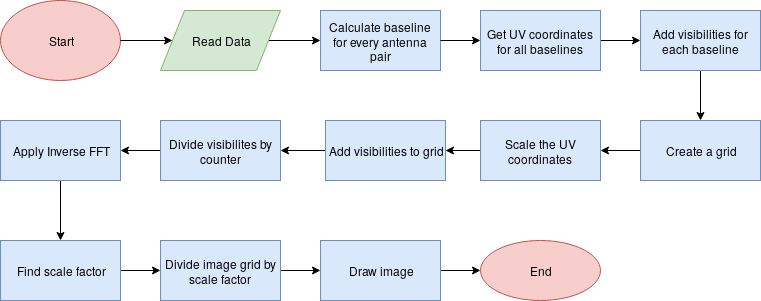
\includegraphics[scale=0.5]{images/FlowDiagram.png}
\end{center}{}
\subsection{Components}
There are three main components: Utilities, Requests and Pipeline.
\begin{center}
    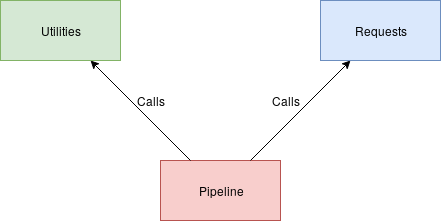
\includegraphics[scale=0.6]{images/BlockDiagram.png}
\end{center}{}
\subsubsection{Utilities}
The utilities component contains all the functions the the imaging pipeline uses.\\
It contains all the code that plots the graphs, it contains all the code that converts from one coordinate system to another. It finds the UV tracks and the visibilities associated with them. For the custom array layout, it determines through Fourier transform the sampled visibilities of the sky model, and then plots them. It uses the cell size and resolution to create a grid of visibilities. It converts the grid of visibilities into an image.\\
The utilities are called by the pipeline component.

\subsubsection{Requests}
The requests component contains the http requests for interfacing with TART, in New Zealand and South Africa, it contains three requests.
\begin{itemize}
    \item \textbf{Antenna Layout} This retrieves the the current antenna layout for the chosen TART interferometer.
    \item \textbf{Visibilities} This retrieves the latest visibilities from the chosen TART interferometer.
    \item \textbf{Latitude and Frequency} This retrieves all the information about TART, but all the pipeline needs is the latitude and frequency so the rest of the information is not used.
\end{itemize}
The requests are called by the pipeline component.

\subsubsection{Pipeline}
The pipeline is where CherryPy interfaces with python. It contains two main functions, one for the custom array layout image generation and one for the TART image generation. \\The custom layout generation takes the cell size, resolution, the baseline the user would like to see, a custom array layout of the users choosing and a sky model of the users choosing as input. It then generates the image for that sky model based off that antenna layout and sky model.\\
The TART image generation function takes the cell size, resolution and which TART interferometer the user would like to use as input. It then generates the image above the specified TART interferomter at that time.

\subsection{Technologies}
The back end is python, implementing libraries found with pip. The front end is a CherryPy web server\cite{Cherrypy} that calls the back end functions and displays the images and plots that are created. The html page that displays the images uses bootstrap\cite{Bootstrap} in order to display the images nicely depending on the layout of the browser.

\section{Testing}
To test the pipeline, the user is able to select their own interferometer to test with, as well as a sky model that has knows positions and brightness.
% functionality was implemented 
% that allows the user to select their own interferometer array layout and sky model.
The user can then generate an image that that interferometer would see if it were to observe that sky model. If the image comes out similar to the sky model then the user knows the pipeline is working as intended. An example is given below: \\
Say the user were to select KAT-7\cite{KAT-7}, which is a real interferometer that we have created a model of to use in our experiments, as the interferometer and select the sky model in figure \ref{fig:line_model}.

\begin{figure}[H]
  \centering
  \begin{subfigure}[b]{0.49\textwidth}
    \centering
    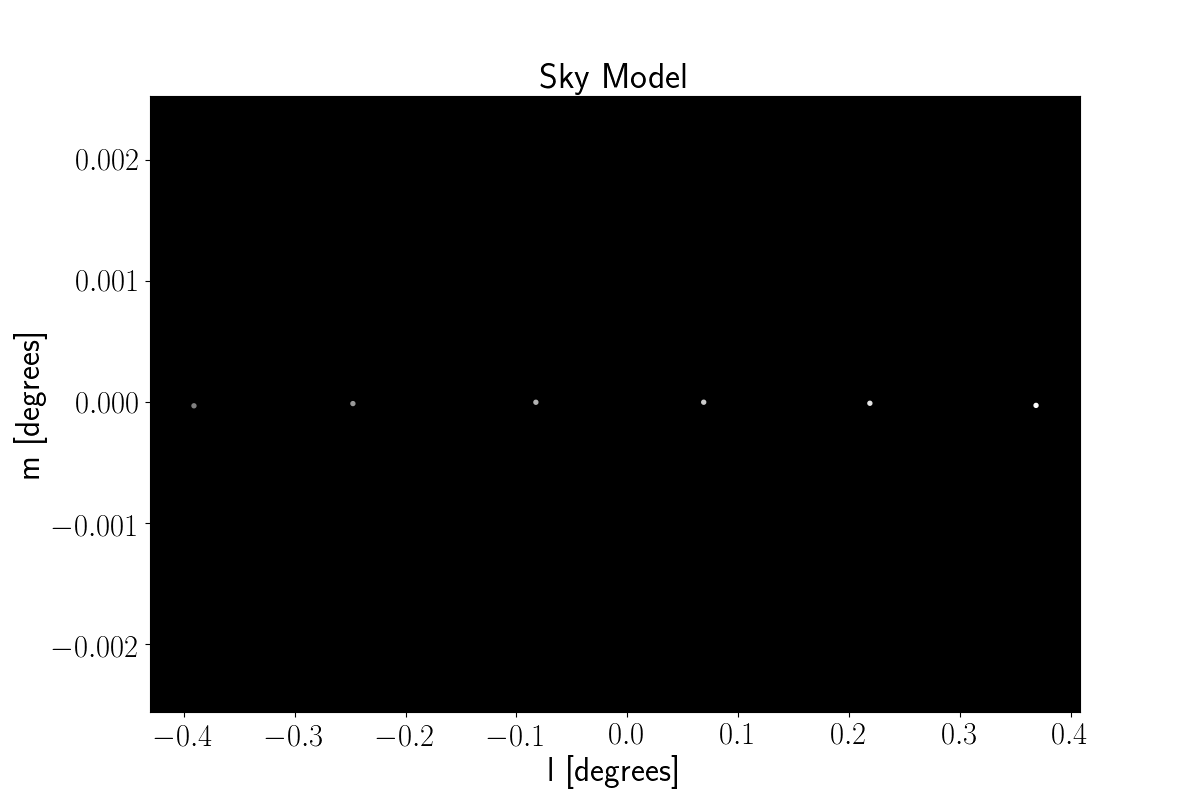
\includegraphics[width=\textwidth, scale=1]{images/TESTING_KAT7_LINEMODEL_SKY_MODEL.png}
    \vspace*{3mm}
    \caption{Testing input.}
    \label{fig:line_model}
  \end{subfigure}
  %
  \begin{subfigure}[b]{0.49\textwidth}
    \centering
    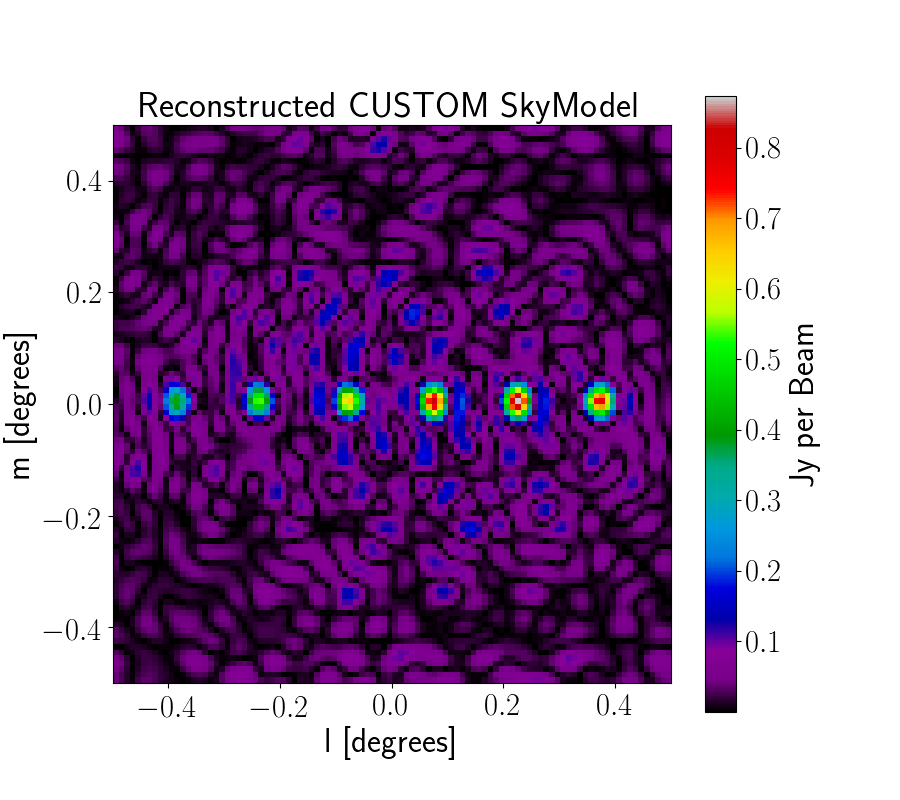
\includegraphics[scale=0.32]{images/TESTING_KAT7_LINEMODEL_RECON.png}
    \vspace*{-8mm}
    \caption{Testing output.}
    \label{fig:line_model_recon}
  \end{subfigure}
  \caption{Testing input and output.}
  \label{fig:Testing}
 \end{figure}

The user would then select a field of view of 1$^\circ$ and a cell size of 0.01$^\circ$.\\
The testing framework will generate an image based off the interferometer and sky model, the output of this testing will be figure \ref{fig:line_model_recon}.

This experiment can be applied to many interferometers, real or imaginary with any sky model, and provided the cell size and field of view are chosen correctly, the testing framework will produce an image that closely resembles the original sky model.\\
This shows that the pipeline is working correctly and that the images that are created by the TART section are correct.


\section{Results}
% Example results
\subsection{Simulation Outline}
The simulation results are images that were created using a specific interferometer layout and a specific sky model. The sky model that was used for the following results was a sky model with 4 points, each of which having a different brightness, or flux. The sky model can be seen below. 
\begin{center}
    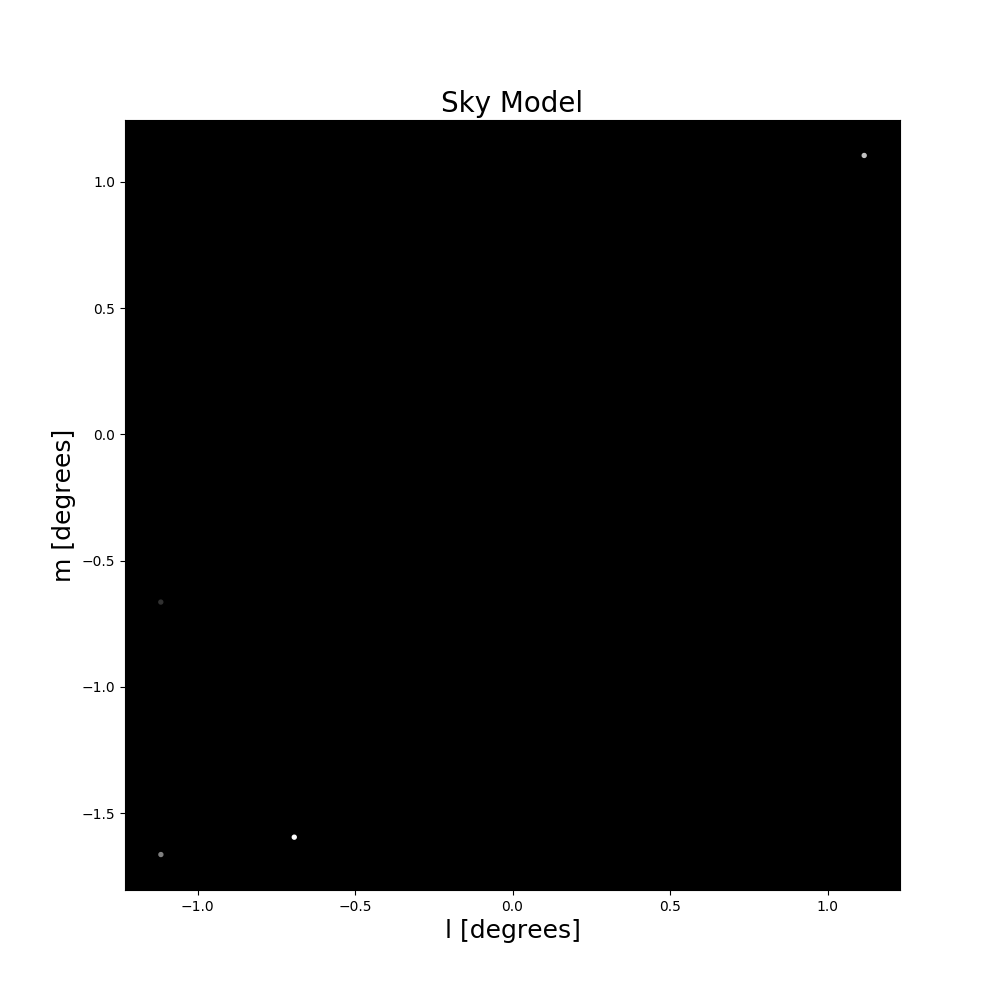
\includegraphics[scale=0.4]{images/4_POINT.png}
\end{center}
The sky model has a distinctive shape to it, the results from each interferomter should have this shape with a point spread function creating some noise around every point source. \\
Before the results are shown, the point spread functions for KAT 7, HERA 19 and TART will be displayed. These are the interferomters that were used to display the results, the TART interferometer here is a antenna layout that was created from TART's actual layout, it is simple treated here as a tracking array, while in reality it is in fact, not a tracking array.
\begin{figure}[htp]
  \centering
  \begin{subfigure}[b]{0.3\textwidth}
    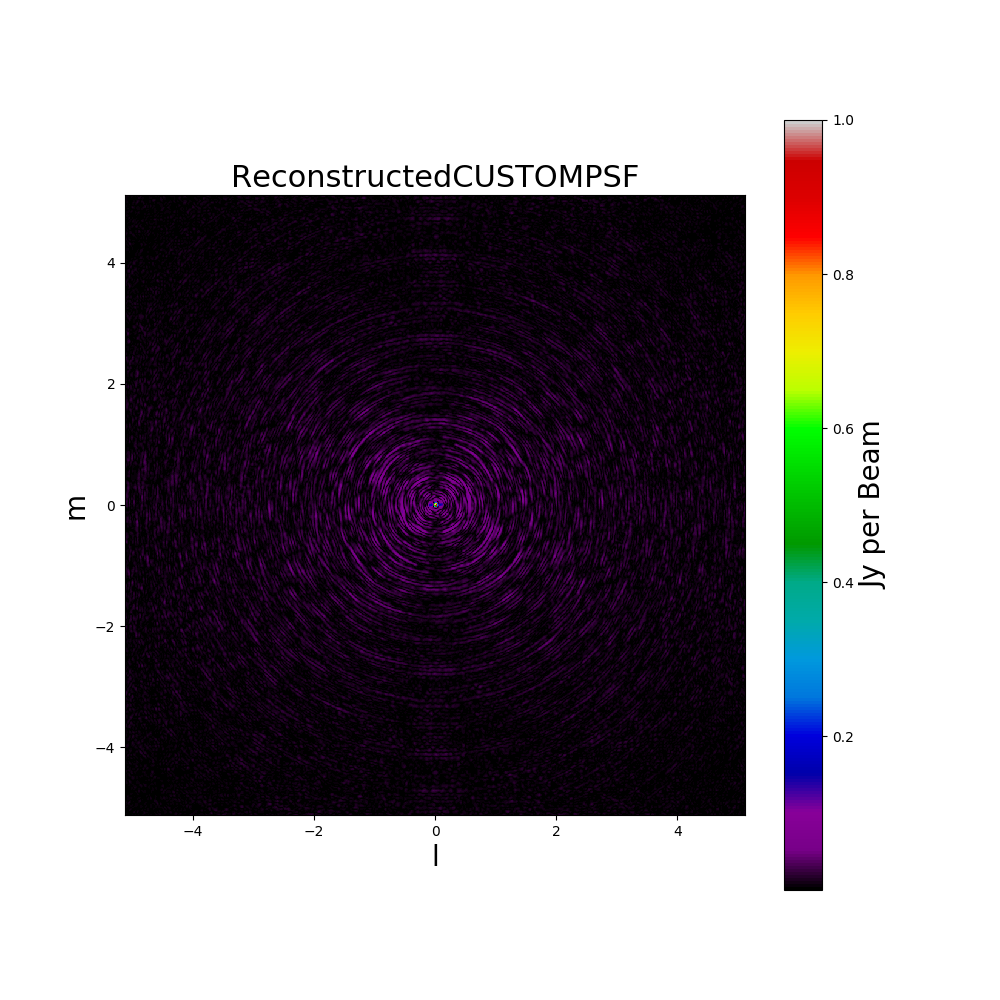
\includegraphics[width=\textwidth]{images/KAT_7_PSF.png}
    \caption{KAT 7 PSF}
    \label{fig:1}
  \end{subfigure}
  %
  \begin{subfigure}[b]{0.3\textwidth}
    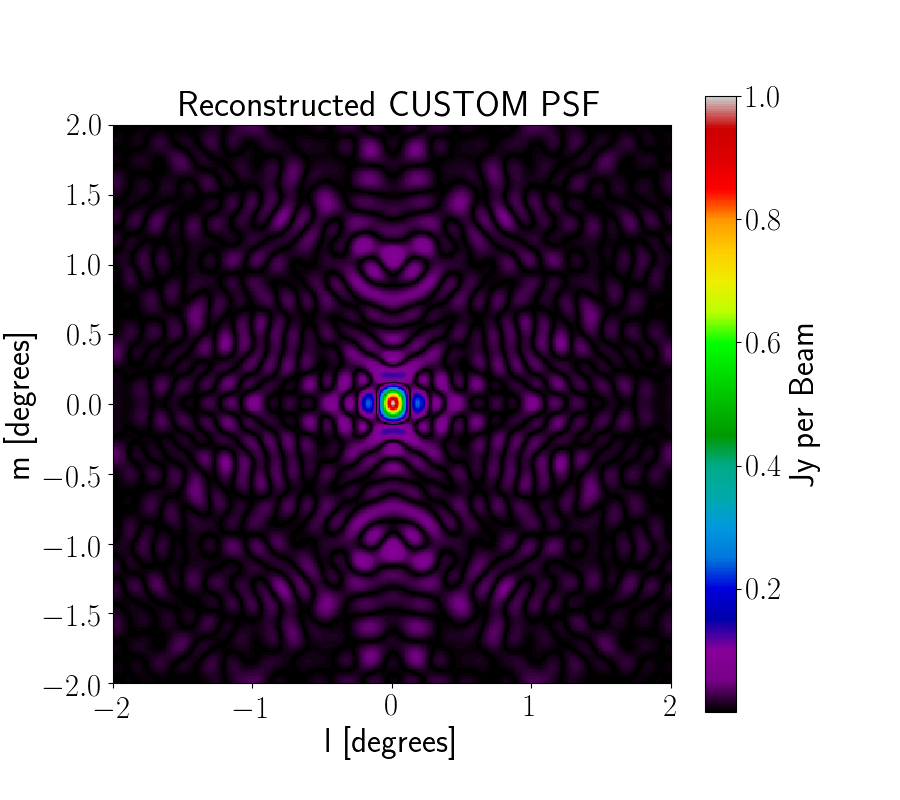
\includegraphics[width=\textwidth]{images/HERA_19_PSF.png}
    \caption{HERA 19 PSF}
    \label{fig:2}
  \end{subfigure}
  %
  \begin{subfigure}[b]{0.3\textwidth}
    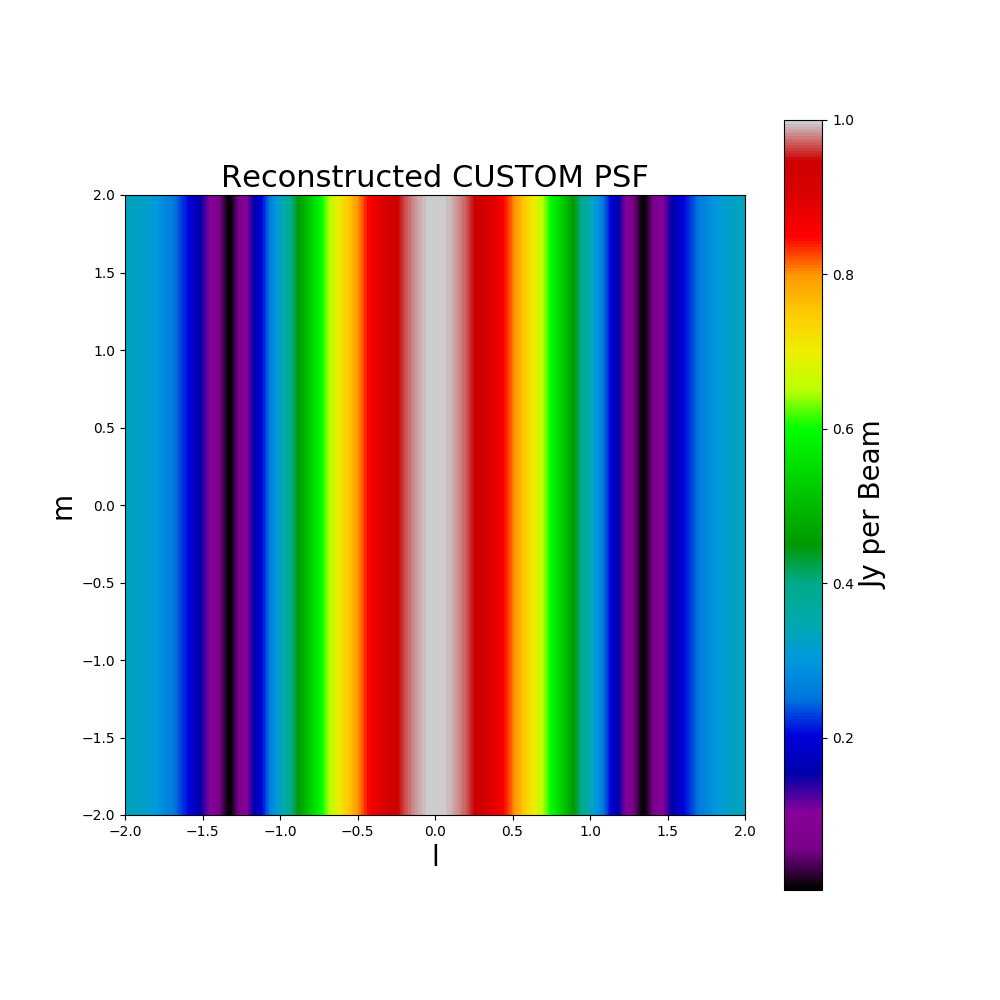
\includegraphics[width=\textwidth]{images/TART_PSF.png}
    \caption{TART PSF}
    \label{fig:2}
  \end{subfigure}
\end{figure}
\subsection{Simulation Results}
Below is a reconstruction from KAT 7 for this sky model using a cell size of $0.01^\circ$ and a resolution of $10^\circ$. 
\begin{center}
    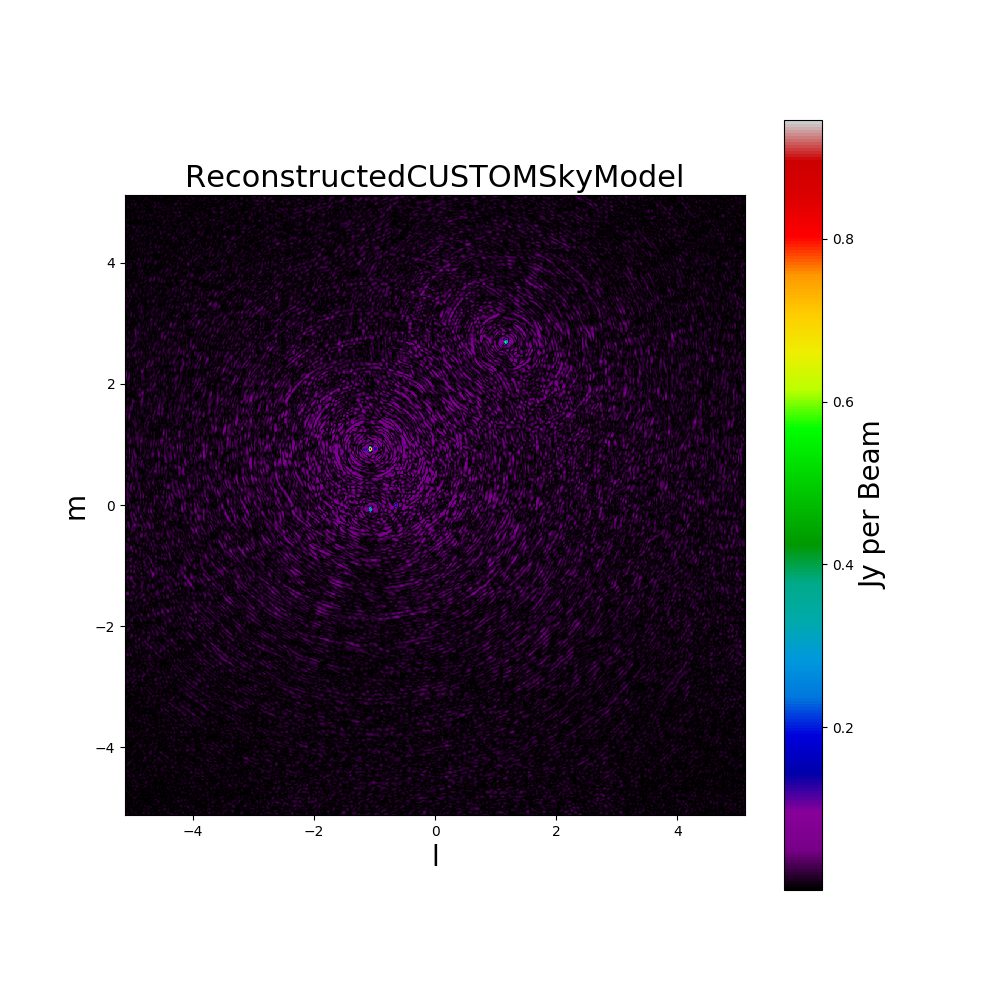
\includegraphics[scale=0.4]{images/RECON_KAT_7_4_POINT.png}
\end{center}
In this image it can be seen that the brighter sources are easily visible, but the one source that was not as bright is not nearly as visible.  The shape is correct and it can clearly be seen that the point spread function has introduced noise to the image and that it matches the point spread function that was introduced earlier in this section.\\
Below is a reconstruction from KAT 7 for this sky model using a cell size of $0.01^\circ$ and a resolution of $3^\circ$. 
\begin{center}
    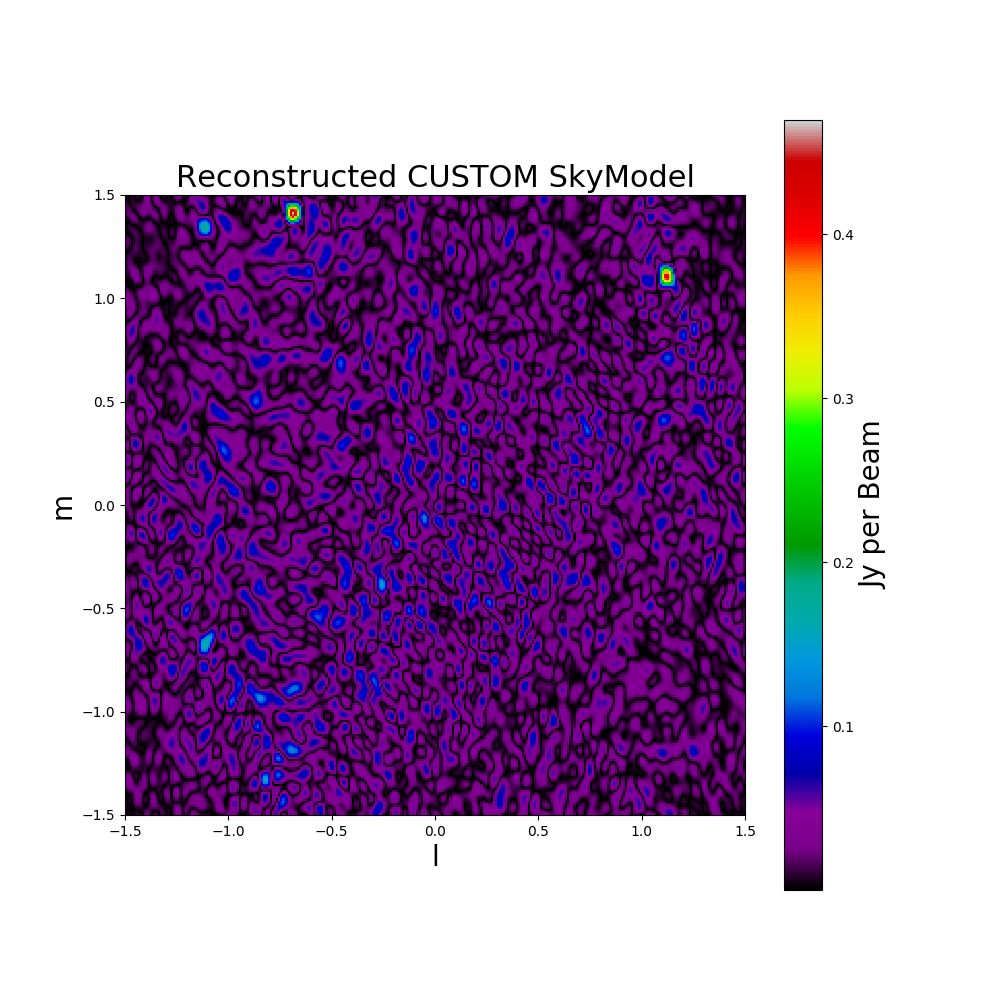
\includegraphics[scale=0.4]{images/RECON_KAT_7_4_POINT_ALIASING.png}
\end{center}
In this image the source at the top appears to be in the wrong location, this is due to aliasing as the resolution was not correctly selected. It is important to remember to follow the Nyquist Theorem that is outlined in section 2.4.1.

Below is a reconstruction from HERA 19 for the sky model using a cell size of $0.01^\circ$ and a resolution of $10^\circ$. 
\begin{center}
    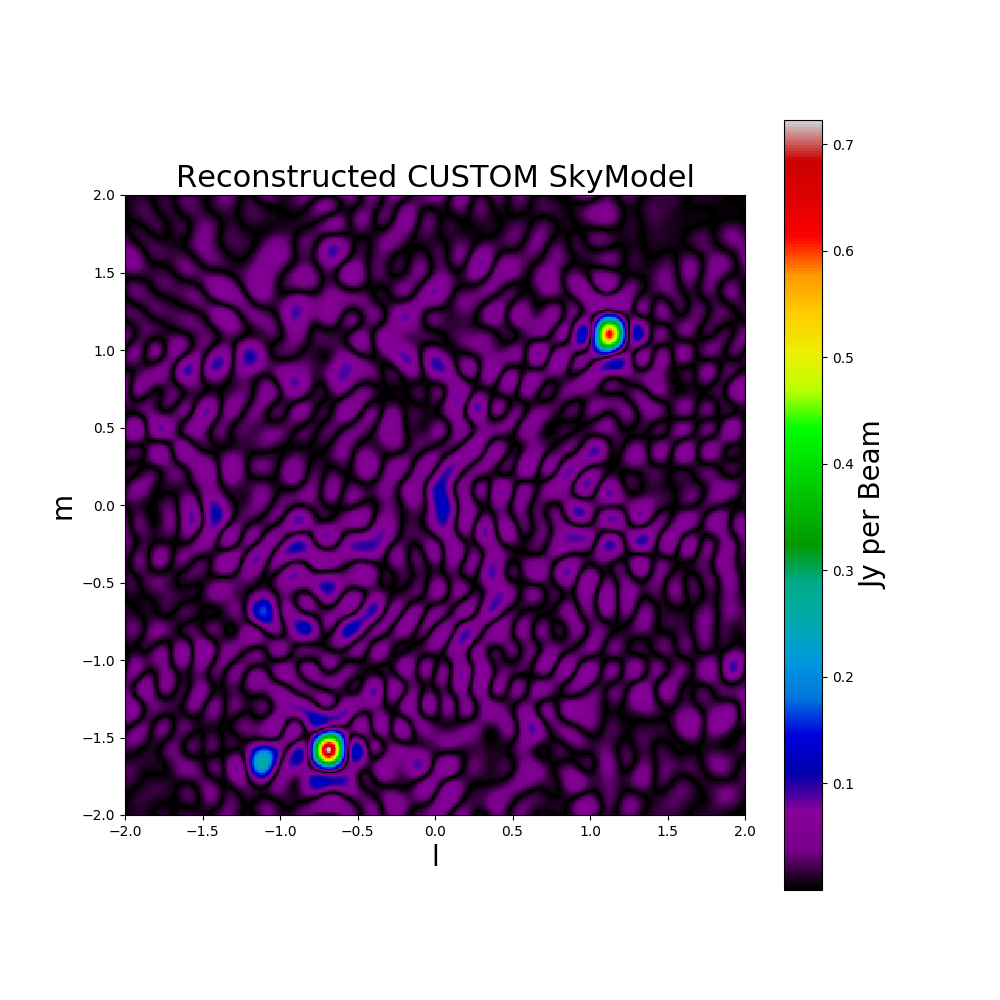
\includegraphics[scale=0.4]{images/RECON_HERA_19_4_POINT.png}
\end{center}
As with the KAT 7 image, the bright sources are easily visible while the one less bright source is hard to identify. The point spread function has introduced noise to the image around the sources and it is clear that it is the same point spread function that was shown earlier in this section.

Below is a reconstruction from TART for the sky model using a cell size of $0.01^\circ$ and a resolution of $10^\circ$. 
\begin{center}
    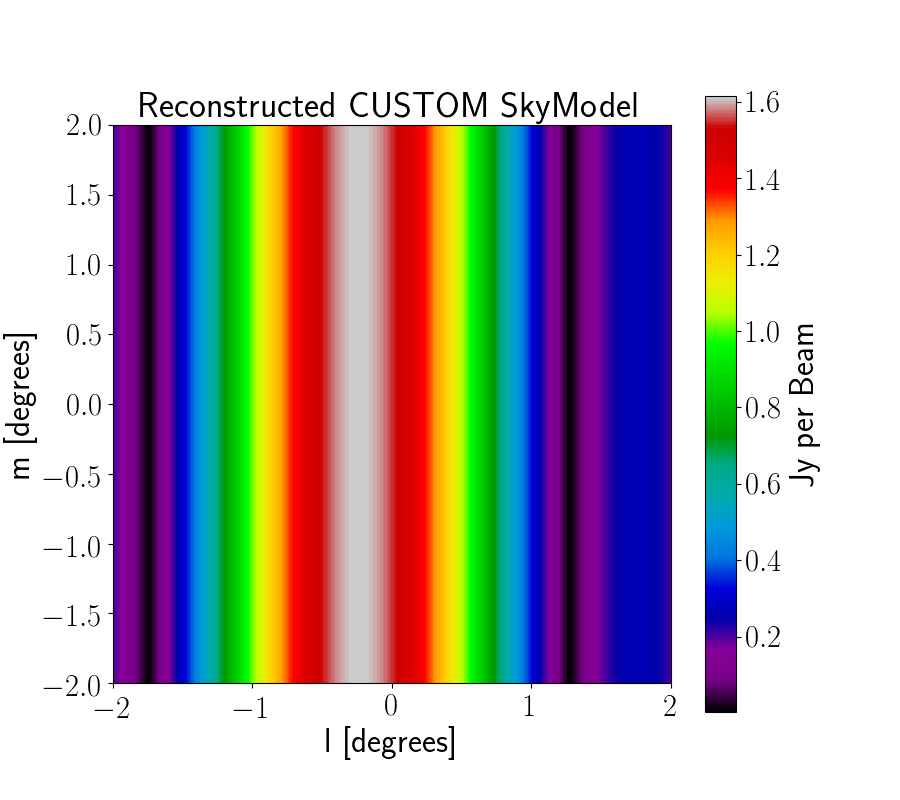
\includegraphics[scale=0.4]{images/RECON_TART_4_POINT.png}
\end{center}
It is instantly clear that the points are not at all visible in this reconstruction, this is because TART is not nearly as powerful as KAT 7 or HERA 19, it is also due to the very small hour angle that was given to TART for this simulation.

\subsection{TART Images}

\subsection{Conclusion}
The pipeline works correctly if the correct resolution is chosen for the images and if the user selects the correct cell size.\\
The images obtained from TART do not show much detail as TART is not a very powerful interferometer. As such, the results that are obtained from it will never match what is being produced by larger projects. So images will never show high levels of detail. TART is also a whole sky interferometer, this also means that the images are less detailed as they don't focus on a small area of the sky which would allow for higher details.
% It is however a perfect tool to teach students how radio interferometry works and if this pipeline was turned into a teaching tool it could explain the subject matter while having a real interferometer to show results with.

% Show simulation
%  Image from TART as final result

\section{Future Work}
\subsection{Calibration}
The TART interferometer needs to have a calibration step applied to it before it can be used to create images, otherwise the images it creates will not be completely correct. The calibration step can be done by creating a source with a strong radio signal nearby, for instance on top of a mountain near Stellenbosch that the interferometer can detect a strong signal from. This signal can then be used as a base for calibrating the interferometer as there is a source with a known signal strength.\\
Another method of calibration would be to use the positions of GPS satellites as sources with known signal strength and location\cite{CALIBRATION_TART}. This would work in a similar way to the previous method and is known as self calibration. 
\subsection{Deconvolution}
The TART interferometer needs a step after the imaging process that reduces the noise that is in the image. This noise comes in the form of the point spread function. The deconvolution step will reduce and perhaps remove the point spread function from the image. This will allow only the actual sources that are detected to be displayed and the image will be much clearer to the user.
\subsection{Transform the pipeline into a teaching tool}
This will allow the pipeline to teach people who are interested in interferometry about how it all works. 
The goal is to create a tool that can be used at a university level to teach students about interferometry in a way where they have access to a working interferometer and a pipeline that will explain every step in high detail to the student. Each step will explain the theory behind it and explain the process that was followed in that step to produce the results that are seen. Hopefully this will increase the ease of learning for interferometry and make more people interested in the field.
\subsection{Convert the data from TART into measurement set format}
The TART interferometer currently saves files in an HDF format, the goal would be to convert an observation into the measurement set format. This would allow the user to take that data and input it into CASA\cite{CASA}, which would mean that the images from the pipeline can be compared to CASA images. This would allow the teaching tool aspect of the tool to expand even further and teach students better. 

\newpage
\begin{thebibliography}{9}
\bibitem{DefinitionInterferometer} 
National Radio Astronomy Observatory [online] Available at:\\
\url{https://science.nrao.edu/facilities/alma/naasc-workshops/nrao-cd-fit/BasicsInterf.pdf}. \\
$[$Accessed 10 September 2019$]$
\bibitem{DefinitionInterferometer2} 
Swineburne University of Technology [online] Available at:\\
\url{http://astronomy.swin.edu.au/cosmos/R/Radio+Interferometer}. \\
$[$Accessed 10 September 2019$]$
\bibitem{Cherrypy}
Cherrypy Home [online] Available at:\\
\url{https://cherrypy.org/}\\
$[$Accessed 12 September 2019$]$
\bibitem{Bootstrap}
Bootstrap Home [online] Available at:\\
\url{https://getbootstrap.com/}\\
$[$Accessed 14 September 2019$]$
\bibitem{aliasing}
Olshausen, B. (2000). Aliasing. [online] Rctn.org. Available at:\\
\url{http://www.rctn.org/bruno/npb261/aliasing.pdf}\\
$[$Accessed 13 September 2019$]$.
\bibitem{CALIBRATION_TART}
Molteno, T., Scheel, M. and Fox, C. (n.d.). Continuous Calibration of the Transient Array Radio Telescope using Satellites.\\
$[$Accessed 16 October 2019$]$
\bibitem{DESIGN_TART}
Shaw, C., Scheel, M. and Molteno, T. (n.d.). Transient Array Radio Telescope: Design.\\
$[$Accessed 16 October 2019$]$
\bibitem{CALIBRATION_AND_SYNTHESIS_TART}
Molteno, T., Scheel, M. and Fox, C. (n.d.). Continuous Calibration of the Transient Array Radio Telescope using Satellites.\\
$[$Accessed 16 October 2019$]$
\bibitem{LAYOUT_TART}
Scheel, M. and Molteno, T. (n.d.). Antenna Array Layout for the Transient Array Radio Telescope.\\
$[$Accessed 16 October 2019$]$
% \bibitem{PHD_TART}
% Scheel, M. (1988). Instrumentation and Calibration of the Transient Array Radio Telescope. Ph.D. University of Otago.
% $[$Accessed 16 October 2019$]$
\bibitem{RADIO_CHIP}
MAX2769B Universal GPS receiver [online] Available at\\
\url{https://datasheets.maximintegrated.com/en/ds/MAX2769B.pdf}\\
$[$Accessed 16 October 2019$]$
\bibitem{TEXTBOOK}
Fundamentals of Interferometry. [online] Avaivable at\\
\url{https://github.com/ratt-ru/fundamentals_of_interferometry}
$[$Accessed 1 March 2019$]$
\bibitem{CASA}
National Radio Astronomy Observatory [online] Available at\\
\url{https://casa.nrao.edu/}
$[$Accessed 24 October 2019$]$

\end{thebibliography}


\end{document}